\let\negmedspace\undefined
\let\negthickspace\undefined
\documentclass[journal,12pt,onecolumn]{IEEEtran}
\usepackage{cite}
\usepackage{amsmath,amssymb,amsfonts,amsthm}
\usepackage{algorithmic}
\usepackage{graphicx}
\usepackage{textcomp}
\usepackage{xcolor}
\usepackage{txfonts}
\usepackage{listings}
\usepackage{enumitem}
\usepackage{mathtools}
\usepackage{gensymb}
\usepackage{comment}
\usepackage{caption}
\usepackage[breaklinks=true]{hyperref}
\usepackage{tkz-euclide} 
\usepackage{listings}

\usepackage{gvv}                                        
%\def\inputGnumericTable{}                                 
\usepackage[latin1]{inputenc}     
\usepackage{xparse}
\usepackage{color}                                            
\usepackage{array}                                            
\usepackage{longtable}                                       
\usepackage{calc}                                             
\usepackage{multirow}
\usepackage{multicol}
\usepackage{hhline}                                           
\usepackage{ifthen}                                           
\usepackage{lscape}
\usepackage{tabularx}
\usepackage{array}
\usepackage{float}
%\newtheorem{theorem}{Theorem}[section]
%\newtheorem{theorem}{Theorem}[section]
%\newtheorem{problem}{Problem}
%\newtheorem{proposition}{Proposition}[section]
%\newtheorem{lemma}{Lemma}[section]
%\newtheorem{corollary}[theorem]{Corollary}
%\newtheorem{example}{Example}[section]
%\newtheorem{definition}[problem]{Definition}

\begin{document}

\title{8.3.15}
\author{AI25BTECH11035 - SUJAL RAJANI}
% \maketitle
% \newpage
% \bigskip
%\begin{document}
{\let\newpage\relax\maketitle}
%\renewcommand{\thefigure}{\theenumi}
%\renewcommand{\thetable}{\theenumi}
% \newpage
% \bigskip
\textbf{Question:} Find the roots of the following quadratic equation graphically:
\[
16x^2 - 8x + 1 = 0
\]

\textbf{Solution:}

First, we expand and observe that the equation is already in standard quadratic form:
\[
16x^2 - 8x + 1 = 0
\]

\textbf{Input Variables:}

The given quadratic can be written in the conic form:
\[
\vec{x}^T\vec{V}\vec{x} + 2\vec{u}^T\vec{x} + f = 0
\]
where
\[
\vec{V} = \begin{pmatrix} 16 & 0 \\ 0 & 0 \end{pmatrix}, \quad
\vec{u} = \begin{pmatrix} -4 \\ 0 \end{pmatrix}, \quad
f = 1
\]

Since the roots correspond to intersections with the x-axis, we represent the line:
\[
L : \vec{x} = \vec{h} + \kappa\vec{m}
\]
with
\[
\vec{h} = \begin{pmatrix} 0 \\ 0 \end{pmatrix}, \quad
\vec{m} = \begin{pmatrix} 1 \\ 0 \end{pmatrix}
\]

\begin{longtable}{|c|c|}
\hline
\textbf{Symbol} & \textbf{Value} \\
\hline
$\vec{V}$ & $\begin{pmatrix} 16 & 0 \\ 0 & 0 \end{pmatrix}$ \\
\hline
$\vec{u}$ & $\begin{pmatrix} -4 \\ 0 \end{pmatrix}$ \\
\hline
$f$ & $1$ \\
\hline
$\vec{h}$ & $\begin{pmatrix} 0 \\ 0 \end{pmatrix}$ \\
\hline
$\vec{m}$ & $\begin{pmatrix} 1 \\ 0 \end{pmatrix}$ \\
\hline
\end{longtable}

The points of intersection of a line with a conic are given by:
\[
\kappa = \frac{1}{\vec{m}^T\vec{V}\vec{m}}
\left[
-\vec{m}^T(\vec{V}\vec{h}+\vec{u}) \pm 
\sqrt{
\left[
\vec{m}^T(\vec{V}\vec{h}+\vec{u})
\right]^2 - g(\vec{h})\vec{m}^T\vec{V}\vec{m}
}
\right]
\]
where
\[
g(\vec{h}) = \vec{h}^T\vec{V}\vec{h} + 2\vec{u}^T\vec{h} + f
\]

\textbf{Step 1: Compute $\vec{m}^T\vec{V}\vec{m}$}
\[
\vec{m}^T\vec{V}\vec{m} = 16
\]

\textbf{Step 2: Compute $\vec{V}\vec{h} + \vec{u}$}
\[
\vec{V}\vec{h} + \vec{u} = \begin{pmatrix} 0 \\ 0 \end{pmatrix} + \begin{pmatrix} -4 \\ 0 \end{pmatrix} = \begin{pmatrix} -4 \\ 0 \end{pmatrix}
\]

\textbf{Step 3: Compute $\vec{m}^T(\vec{V}\vec{h}+\vec{u})$}
\[
\vec{m}^T(\vec{V}\vec{h}+\vec{u}) = (1,0) \cdot (-4,0) = -4
\]

\textbf{Step 4: Compute $g(\vec{h})$}
\[
g(\vec{h}) = 0 + 0 + 1 = 1
\]

\textbf{Step 5: Substitute into formula for $\kappa$}
\[
\kappa = \frac{-(-4) \pm \sqrt{(-4)^2 - 16 \cdot 1}}{16}
= \frac{4 \pm \sqrt{16-16}}{16}
= \frac{4}{16}
= 0.25
\]

\textbf{Step 6: Find intersection point}

The intersection is 
\[
x = h + \kappa m = (0,0) + (0.25)(1,0) = (0.25, 0)
\]

Thus, the quadratic $16x^2 - 8x + 1 = 0$ intersects the x-axis at
\[
\boxed{x = 0.25}
\]
      \begin{frame}[fragile]
    \begin{figure}[H]
    \centering
    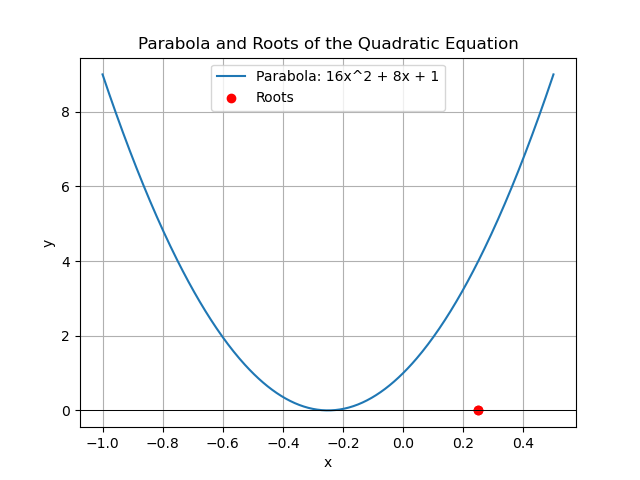
\includegraphics[width = 0.6\columnwidth]{figs/img.png}
    \caption*{}
    \label{figs}
\end{figure}
\end{frame}
\end{document}
